% Created 2016-01-30 Sat 12:20
\documentclass[journal=accacs,manuscript=article,email=true]{achemso}
  \setkeys{acs}{biblabel=brackets,super=true,articletitle=false}
\setkeys{acs}{keywords = true}
\SectionNumbersOn
\usepackage[utf8]{inputenc}
\usepackage{url}
\usepackage[version=3]{mhchem}
\usepackage{graphicx}
\usepackage{float}
\usepackage{subcaption}
\usepackage{tcolorbox}
\usepackage{color}
\usepackage{amsmath}
\usepackage{textcomp}
\usepackage{wasysym}
\usepackage{latexsym}
\usepackage{amssymb}
\usepackage[version=3]{mhchem}
\usepackage{minted}
\usepackage[linktocpage, pdfstartview=FitH, colorlinks, linkcolor=black, anchorcolor=black, citecolor=black, filecolor=black, menucolor=black, urlcolor=black]{hyperref}
\author{John R. Kitchin}
\email{jkitchin@andrew.cmu.edu}
\affiliation{Department of Chemical Engineering, Carnegie Mellon University, 5000 Forbes Ave, Pittsburgh, PA 15213}
\date{}
\title{Examples of effective data sharing in scientific publishing}
\begin{document}

\begin{abstract}
We present a perspective on an approach to data sharing in scientific publications we have been developing in our group. The essence of the approach is that data can be embedded in a human-readable and machine-addressable way within the traditional publishing environment. We show this by example for both computational and experimental data. We articulate a need for new authoring tools to facilitate data sharing, and discuss the tools we have been developing for this purpose. With these tools, data generation, analysis, and manuscript preparation can be deeply integrated, resulting in easier and better data sharing in scientific publications.
\end{abstract}

\textbf{Keywords:} data sharing, org-mode, Emacs, Python, reproducible research

\section{Introduction}
\label{sec-1}
Data sharing and management plans are becoming an increasingly important requirement for scientific research. The National Science Foundation requires a data management plan \cite{foundation-nsf-data} for all proposals and has a formal statement on data sharing \cite{foundation-dissem-sharin}. The Department of Energy is beginning to require this in some proposals and has issued a formal statement on data management \cite{energy-statem-digit}. The National Institutes of Health has a formal data sharing policy \cite{health-nih-data}. These mandates do not usually say how the data management plan must be implemented, simply that there must be one that is appropriate for the data being generated and consistent with the needs of the scientific field.

There are several challenges to meeting these requirements. Data is a generic term that refers to a broad range of information that varies in size and complexity. There is no single solution that fits all data. The tools we use to write manuscripts, which has been the primary mode of data sharing for decades typically only include graphical or tabular data. Those data are usually not machine readable nor are they easy to reuse. We believe that progress in data sharing will require the development of new tools and social expectations about scientific data. These tools will have to integrate data directly into the manuscripts, and into the manuscript preparation workflow so that by the time one finishes writing the manuscript the data is already integrated and ready to share with no further work required. When this is possible, data will be shared much more frequently.

In this viewpoint, we illustrate an example of a method we have been developing that enables data, analysis and code sharing within the traditional publishing environment. We have published several papers this way already including experimental work \cite{hallenbeck-2013-effec-o2}, combined computational and experimental work \cite{miller-2014-simul-temper} and computational work \cite{curnan-2014-effec-concen,xu-2014-probin-cover,xu-2014-relat,mehta-2014-ident-poten}.  These manuscripts in published form are indistinguishable from other manuscripts in those journals. However, the supporting information files are very different. Although at first glance the supporting information files are simple PDF files that provide additional information, there are actually data files embedded (See Fig. \ref{fig-attachments} a) in those PDFs which can be extracted and reused. The data is human readable in most cases, and machine addressable, enabling reuse and sharing. We will provide an example of this for a paper we recently published in ACS Catalysis on "Estimating Bulk-Composition-Dependent \ce{H2} Adsorption Energies  on Cu$_{\text{x}}$Pd$_{\text{1-x}}$ Alloy (111) Surfaces" \cite{boes-2015-estim-bulk}.

\begin{figure}[H]
\centering
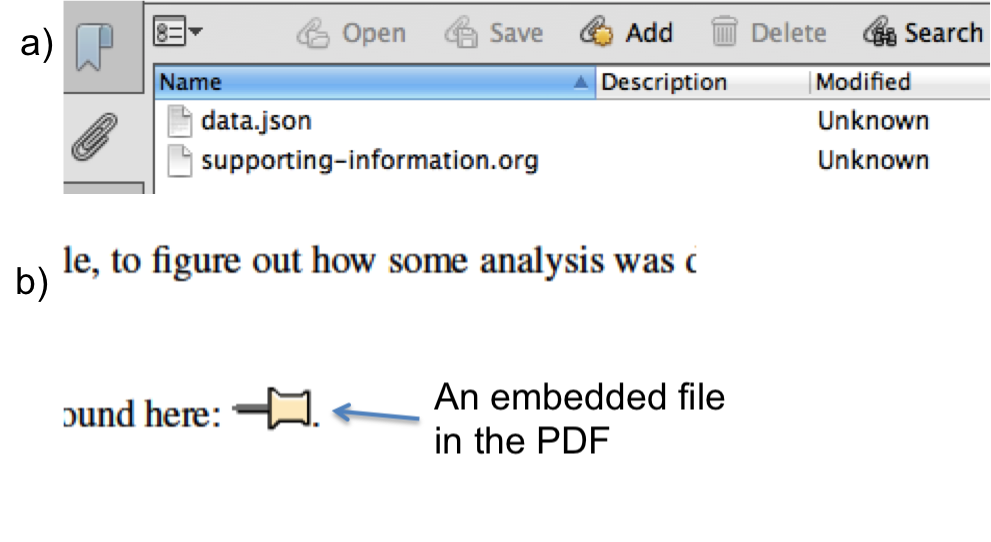
\includegraphics[width=3in]{embedded-attachments}
\caption{a) The attachments in the supporting information of Ref. \citenum{boes-2015-estim-bulk}. There are two attachments. b) A single attachment in the PDF file. Double-clicking on the thumbtack will open the attached file. \label{fig-attachments}}
\end{figure}

The supporting information file for that article is available for free \cite{boes-2015-estim-bulk-si}. When opened in a PDF reader that supports attachments, one can see that there are attachments (see Fig. \ref{fig-attachments} a). Alternatively, while reading the PDF file, the reader is alerted that there is an attachment by the presence of a thumbtack icon (Fig. \ref{fig-attachments} b) which can be double clicked to open the file. An alternative approach to extracting the data and source file is to use a command-line program, pdftk \cite{labs-pdftk} to extract the files from the pdf. File attachments are a standard feature of the PDF specification, and there are a number of ways to create them. This supporting information file has two attachments: one is a JSON data file, and one is the source file that generated the PDF. It is also possible to embed data files in a Word document.

An example of using a command line utility to extract the attachments is shown in Listing \ref{pdftk}, which will extract the two data files into the current directory the command is run in. The contents of the files that are extracted are explained in the supporting information file, which in this case even contains examples of how to use the data.

\begin{tcolorbox}
src block name: pdftk\\language: sh\begin{listing}[H]
\begin{minted}[frame=lines,fontsize=\scriptsize]{sh}
pdftk cs501585k_si_001.pdf unpack_files
\end{minted}
\caption{\label{pdftk}Command line extraction of the attached files in the supporting information PDF.}
\end{listing}
\end{tcolorbox}

This idea of file attachments is one that almost everyone could adopt immediately. File attachments can be added using Adobe Professional, or other PDF editing tools. They can also be added in \LaTeX{} using the attachfile package \cite{pakin-attachfile}. Word documents also support file attachments. This small step could significantly improve data sharing. While some standardization of data formats could be helpful, if this delays sharing, constrains creativity, or limits sharing, we should tolerate non-standard approaches. The shared data that is easiest to use will get used more often than data that is not easy to use.

In the next sections we illustrate how easy it is to do this in a few applications. We will first show an example of an embedded data file and its use. Then, we will show an alternative example, and a more sophisticated approach to data sharing.

\section{Use of an embedded data file}
\label{sec-2}
We embedded a data file (data.json) in the supporting information PDF file. The file is in JSON format. JSON (javascript object notation) is a standard data format often used in web programming. It is structured, and can be read by a number of programming languages, or by web-based programs, e.g.  \url{http://www.jsoneditoronline.org/}. The data set here is a fit-for-purpose format, which is described in the supporting information document.

The data.json file embedded in the supporting information PDF contains all the geometries and computational parameters used for every DFT calculation in the paper. Here, we consider how one could extract the information for a single calculation so that it could be used as the starting point for a new calculation. To do this in VASP, for example, that means extracting the data needed to create an INCAR, POSCAR, POTCAR, and KPOINTS file. These are input files for the VASP density functional theory code. We will choose as the example a clean palladium hydride slab. The critical point we wish to communicate here is that there is machine-readable code \emph{embedded} in the supporting information file that can be reused.

Reading the supporting information file suggests the following Python \cite{python,millman-2011-python-scien-engin,perkel-2015-progr} code (Listing \ref{code-incar}) would extract the INCAR parameters, and then we write each key/value pair to a file called INCAR (a file containing input parameters for VASP). There is an extra key called "doc" which provides some documentation on the data, which we delete before creating the INCAR file. We choose an example of a Pd hydride slab. The terminology that follows is likely to be known to those familiar with VASP. It is not critical that Python be used here, many other languages can accomplish the same result including Perl, Ruby, emacs-lisp, and others. Python loads a json file as a dictionary, which enables data to be looked up as "key:value" pairs. A value can be another dictionary, providing a nested data structure.

\begin{tcolorbox}
src block name: INCAR\\language: python\begin{listing}[H]
\begin{minted}[frame=lines,fontsize=\scriptsize]{python}
import json

with open('data.json', 'rb') as f:
    d = json.loads(f.read())

calc = d['results']['HPd']['cln'][0]
# delete the doc string; it is not part of the incar.
del(calc['incar']['doc'])
with open('INCAR', 'w') as f:
    for key, val in calc['incar'].items():
        f.write('{0} = {1}\n'.format(key.upper(), val))
\end{minted}
\caption{\label{INCAR}A Python script to load a json file and extract information about a calculation. \label{code-incar}}
\end{listing}
\end{tcolorbox}

Now, we have an INCAR file with these contents, which define the parameters VASP will use in the calculation. Listing \ref{code-cat} shows how to view the contents of the INCAR file.

\begin{tcolorbox}
language: sh\begin{listing}[H]
\begin{minted}[frame=lines,fontsize=\scriptsize]{sh}
cat INCAR
\end{minted}
\caption{Shell command to print the contents of the INCAR to the console. \label{code-cat}}
\end{listing}
\end{tcolorbox}

\begin{verbatim}
PREC = Normal
ISIF = 2
IBRION = 2
NBANDS = 156
ENCUT = 450.0
NSW = 30
\end{verbatim}

We can similarly retrieve information about which POTCAR files were used. The VASP license prohibits sharing these, so information about the files used is all one can do here, and to reproduce the calculation requires one to have a VASP license. Note that it will not always be possible to share all data. But, often it is possible to share enough data so that another expert can reproduce the work.

\begin{tcolorbox}
language: python\begin{listing}[H]
\begin{minted}[frame=lines,fontsize=\scriptsize]{python}
import json
import numpy as np

with open('data.json', 'rb') as f:
    d = json.loads(f.read())

calc = d['results']['HPd']['cln'][0]

print 'POTCARS:'
for sym, potcar, githash in calc['potcar']:
    print(sym, potcar, githash)
\end{minted}
\caption{Python script to read the POTCAR file information for a specific calculation.}
\end{listing}
\end{tcolorbox}

\begin{verbatim}
POTCARS:
(u'H', u'potpaw_PBE/H/POTCAR', u'fbc0773b08b32f553234b0b50cc6ad6f5085c816')
(u'Pd', u'potpaw_PBE/Pd/POTCAR', u'abec334aaffe253d3b9fb835c3a06cba6c014023')
\end{verbatim}

The KPOINTS file would be created from data in the "input" section of the calculator data. We extract these in Listing \ref{code-kpoints}. Based on the information provided, it is evident a KPOINTS file should be generated that creates a 10 \texttimes{} 10 \texttimes{} 1 Monkhorst-Pack k-point grid.

\begin{tcolorbox}
language: python\begin{listing}[H]
\begin{minted}[frame=lines,fontsize=\scriptsize]{python}
import json
import numpy as np

with open('data.json', 'rb') as f:
    d = json.loads(f.read())

calc = d['results']['HPd']['cln'][0]

print 'OTHER INPUT:'
for key, val in calc['input'].items():
    print('{0} = {1}'.format(key, val))
\end{minted}
\caption{Python script to read the other calculation parameters such as k-point sampling, and exchange-correlation functional. \label{code-kpoints}}
\end{listing}
\end{tcolorbox}

\begin{verbatim}
OTHER INPUT:
kpts = [10, 10, 1]
reciprocal = False
xc = PBE
kpts_nintersections = None
setups = {}
txt = -
gamma = False
\end{verbatim}

We can leverage the Atomic Simulation Environment (ASE) \cite{bahn-2002} to easily create the POSCAR file from the chemical symbols, positions, and unit cell stored in the json file. ASE can also write other input file types including GPAW, Wien2K, Castep, Siesta, Turbomol, FHI-AIMS, Gaussian, and Quantum Espresso, in addition to file formats such as CUBE, xyz, cif, and some database formats. Once the information is in Python, as we use below, one can write code to convert the information to nearly any format desired. In Listing \ref{code-poscar} we generate a POSCAR file (the file containing atomic coordinates and unit cell for the VASP code). The generated POSCAR file is somewhat long, so we do not show it here.

\begin{tcolorbox}
language: python\begin{listing}[H]
\begin{minted}[frame=lines,fontsize=\scriptsize]{python}
import json
import numpy as np
from ase import Atom, Atoms
from ase.io import write
from ase.visualize import view

with open('data.json', 'rb') as f:
    d = json.loads(f.read())

calc = d['results']['HPd']['cln'][0]

atoms = Atoms([Atom(str(sym), pos) for sym,pos in zip(calc['atoms']['symbols'],
                                                 calc['atoms']['positions'])],
              cell=calc['atoms']['cell'])

write('POSCAR', atoms)
\end{minted}
\caption{Python script to create a POSCAR file from the json data file for a specific calculation. \label{code-poscar}}
\end{listing}
\end{tcolorbox}

Next, one would then create a POTCAR file (this file contains the pseudopotentials used by VASP)  consistent with the POSCAR file, and then VASP could be run to reproduce the result, or the atoms could be modified to start some new calculation. This JSON file contains all of the data used in making the figures in the paper, and it can all be extracted for reuse using any kind of scripting language with JSON support. It should be evident that this information is sufficient for an expert to create very similar calculations in other DFT codes besides VASP as well.

We emphasize here that JSON was used as a data format because it is 1) suitable to organize the data, 2) it is easy to generate, 3) it is easy to reuse.  However, other data formats are easily used as well. In Ref. \citenum{curnan-2014-effec-concen} we embedded csv (comma-separated value) files. Other formats including netCDF, HDF, sqlite, etc\ldots{} could also be used if they were fit for purpose. It is even possible to embed data files from proprietary softare; in Ref. \citenum{hallenbeck-2013-effec-o2} we embedded Excel files into the supporting information files. Naturally, these files are only useful to people who have access to the software required to read the files.

While it is technically possible to embed any type of file in a PDF, some readers restrict what you are allowed to open. For example, Adobe Acrobat will not allow one to open executable or zip files for security reasons. These can still be extracted using the pdftk software. Alternatively, these files could be provided separately from the PDF supporting information file.

This approach of data file embedding may become impractical for very large datasets. In Ref. \citenum{xu-suppor} we archived a large data set ($\approx$ 1.8 Gb) of DFT calculations in an external data sharing site which assigned the data set a DOI \cite{xu-suppor}. An alternative data repository could be an institutional data repository which also provides a DOI for citing. It remains to be seen if these repositories remain archival quality repositories, and what happens to the data if the repositories cease to operate due to lack of funding or other reasons.

Finally, the embedded data file is part of the supporting information file. The supporting information is in a sense the metadata that informs the reader what is in the file, how it was made, and by example, how to use it.

\section{Embedding data within text}
\label{sec-3}

There is another approach to storing data in the supporting information than just attaching a data file. One challenge with data files is they are often not self-documenting. This means when they are separated from the source, it may not be clear what is in the file, or how to use it. An alternative approach we have been investigating is that the data can be stored in a machine addressable table or code block within the manuscript. Notably, this table is different than what is read by humans in the PDF. Instead, the table is in a source file that is embedded in the PDF. This is the other file named supporting-information.org in our example.  This file is in a plain text format that is lightly marked up using org-mode \cite{Dominik201408} to differentiate text from data and code. When this file is opened in Emacs \cite{emacs}, a powerful text editor, then new data sharing and reuse possibilities are available.

Org-mode is a few different things. First, it is a document markup syntax that is approximately plain text, and that differentiates text, citations, equations, tables, images, code and data. Second, org-mode is a library of code in Emacs that provides rich, functional links, an outline mode, and a capability to embed interactive code and data in a document, and the capability to export the document to another format, e.g. PDF, \LaTeX{}, and html among others. We actually write our scientific papers using org-mode as mentioned already.

Others have also published papers using org-mode, and about org-mode \cite{schulte-2011-activ-docum,schulte-2012-multi-languag}. This manuscript was prepared in org-mode. The code blocks shown in this manuscript are literally the code that was run in the document in each example. Emacs is able to run the codes, capture the output and insert it into the manuscript. Emacs and org-mode are open-source software, available for free on every major computing platform. One does not need Emacs to read org-mode; the format is in plain text. We would never consider writing org files without Emacs; Emacs provides all the functionality that makes org-mode useful for this application. There is limited support for org-mode in other editors. There are limited, but developing, org-mode parsers available in Ruby (e.g. Github can render org files as HTML), and other languages. We will show in the next paragraph that it is possible to read org-mode with other languages. But, to adapt a quote by Neal Stephenson \cite{Stephenson199911}, when it comes to org-mode, "emacs outshines all other editing software in approximately the same way that the noonday sun does the stars. It is not just bigger and brighter; it simply makes everything else vanish."

The key example we want to illustrate here is that tables in org-mode have actually two different functions.  First, they are human-readable, and can be rendered as regular tables in the PDF or html format. Second, they are machine addressable, and can serve as data sources for code blocks. Much of the data used in Ref. \citenum{boes-2015-estim-bulk} is stored in tables in the org-source. org-mode provides native support to read these tables in as an array. Alternatively, one can use any scripting tool to parse the org-file and extract the data. For example, in Listing \ref{read-an-org-file}, we illustrate a small Python code that opens an org-file, finds the table, and returns the data in the table for further analysis. The key point here is that the data is machine readable, and one is not tied to Emacs or org-mode necessarily to take advantage of the embedded data. org-mode is a syntax, which can be parsed by other tools.


\begin{tcolorbox}
src block name: read-an-org-file\\language: python\begin{listing}[H]
\begin{minted}[frame=lines,fontsize=\scriptsize]{python}
def string_to_number(s):
    'Try to convert S to a number, return S otherwise.'
    if '.' in s:  # possible float
        try:
            return float(s)
        except ValueError:
            return s
    else:
        try:
            return int(s)
        except ValueError:
            return s
    return s

def read_org_table(filename, tablename, include_header=True):
    '''Read the table named TABLENAME from the org-file named FILENAME.
    If not INCLUDE_HEADER, skip the first row of the table.'''
    with open(filename) as f:
        contents = f.readlines()
    # find the table name. Starts with a line like #+tblname:
    for i, line in enumerate(contents):
        if (line.lower().startswith('#+tblname')
            and tablename in line):
            table_name = i
            break

    # now find start of data
    table_data_start = table_name
    for line in contents[i:]:
        if line.startswith('|'):
            break
        else:
            table_data_start += 1

    # now read the data
    data = []
    for line in contents[table_data_start:]:
        if not line.startswith('|'):
            break
        elif line.startswith('|-'):
            continue
        row = [string_to_number(x.strip()) for x in line.strip().split('|')]
        data += [row[1:-1]]

    if include_header:
        return data
    else:
        return data[1:]
\end{minted}
\caption{\label{read-an-org-file}Prototype code to read data tables from an org-file. This code is stored in an external Python module named py\_org\_table.py so it can be used by python scripts for analysis.}
\end{listing}
\end{tcolorbox}

We use the code from Listing \ref{read-an-org-file} in Listing \ref{segregation-data} to  show that one can import the data from a table in the supporting information file, and use the data for new uses. We import a table named \texttt{jm-seg} which contains data about the experimentally measured surface and bulk composition of an alloy surface. We use this data to plot the surface composition vs. the bulk composition (Fig. \ref{fig-segregation}). It should be evident that further analysis is possible at this point, using \emph{exactly the same data} as was used in our manuscript.



\begin{tcolorbox}
src block name: segregation-data\\language: python\begin{listing}[H]
\begin{minted}[frame=lines,fontsize=\scriptsize]{python}
from py_org_table import *
import matplotlib.pyplot as plt

data = read_org_table('supporting-information.org', 'jm-seg', False)

bulk_comp = [row[0] for row in data]
surf_comp = [row[1] for row in data]

plt.figure(figsize=(3,4))
plt.plot(bulk_comp, surf_comp)
plt.plot([0, 1], [0, 1], 'k--')
plt.xlabel('$x_{Cu, bulk}$')
plt.ylabel('$x_{Cu, surface}$')
plt.legend(['Expt.', 'parity'], loc='best')
plt.tight_layout()
plt.savefig('images/segregation.png')
\end{minted}
\caption{\label{segregation-data}Example code for extracting tabular data from a supporting information org-file.}
\end{listing}
\end{tcolorbox}

\begin{figure}[htb]
\centering
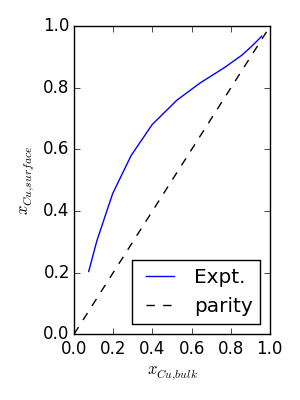
\includegraphics[width=3in]{segregation}
\caption{Experimentally determined surface composition as a function of bulk composition at 900K. \label{fig-segregation}}
\end{figure}

This example brings up an interesting issue. One does not directly measure these compositions. These compositions were derived from XPS and ion scattering experiments. We did not share that data because at the time it was not practical. In Ref. \citenum{miller-2014-simul-temper} the raw temperature programmed desorption spectra can be found in the supporting information org file, but not in the PDF. Including them in the PDF would have made it hundreds of pages long of tabular data. Embedding the tables in the org-file, so they could be used as data sources within the org-file, and then subsequently embedding the org file in the PDF still makes this data available. Alternatively, the data could be shared by external \cite{zenodo-zenod,figshare,the-datav-projec} or institutional data stores that provide a citable DOI for the data set. The point is that this approach is very flexible and allows a broad range of data sharing strategies that can be adapted as appropriate to the sharing need. We are increasingly integrating org-mode into our manuscript preparation workflow, so that the data is already embedded as the manuscript is developed.

\section{Perspective on these approaches}
\label{sec-4}
The first approach we outlined is immediately accessible to nearly every author. Within supporting information files authors could attach data files and explain how to use them. Ideally, the data files are the same files used in making the figures for the manuscript. Attaching files can be tedious if there are many of them, or if one has to reattach files on every iteration of a PDF generation. Tools such as \LaTeX{} make that less tedious by integrating the attachment process in the manuscript build process. Neither of these approaches, however, enable facile inclusion of analysis and code in a way that ensures they are synchronized (i.e. if one copies code into \LaTeX{}, it is no longer guaranteed to be exactly the code that was run to get some results). When coupled with the fact that it is difficult to use the data in the published versions (PDF or html) of manuscripts, these factors among others \cite{borgman-2012} have lead to the dearth of practical data sharing strategies today.

We have illustrated how org-mode can streamline the integration of narrative text, data, analysis and code into manuscripts. It is ultimately a fail-safe approach to data sharing because the data is almost always in human readable, but machine-addressable, form. We recognize that there is a learning curve associated with writing manuscripts this way, but it can be a long and shallow curve that grows with an author. org-mode is not more difficult to learn than \LaTeX{}, and Emacs can be made similar to using Microsoft Word with GUIs and menus. Scientific publishing is a career long activity, and one should not shy away from learning a tool that can have impact over this time scale. If more manuscripts were written in org-mode, the manuscripts themselves would serve as learning opportunities about how to effectively organize data and code for sharing and publications.

The way we use org-mode is essentially like a scientific notebook. Other tools have similar functionality. For example, Matlab has a "notebook" feature that integrates with Microsoft Word \cite{mathworks-matlab-noteb}, as well as functionality to export a Matlab script to HTML or \LaTeX{}. There is the Ipython notebook \cite{perez-2007-ipyth}, which provides similar capability through a web browser, and the newer project Jupyter \cite{projec-juypy} which extends the Ipython concept to other languages. For specific uses, each of these tools may provide a solution similar to what we have described here. None of them, however, have the flexibility and power of org-mode.

It is worth considering the role of standardization in data sharing.  No standard can meet everybody's needs in experimental and computational science.  Even with a standard, the lack of tools in standard authoring tools will limit its use. Our opinion is that we should just start sharing data as we have described in this manuscript. Any sharing would probably be better than the general lack of sharing that occurs today. It is true there may be many different formats, and that some will be better than others. The data that is most valuable will be reused in new forms, and best practices will emerge. Data that is not reused will fade into obscurity, an old tradition in the scientific literature.

This approach is distinctly different than any approach that advocates for a centralized database. In this approach the data is distributed among the publishers, and anyone who downloads the files. Individual users within domains could curate collections of the data that is fit for specific purposes. These domain experts would be able to convert the various formats into a common format used in their research, and likely reshared through the same mechanisms. In contrast, a centralized database would contain a trove of data that is not useful to the majority of the users. Further compounding this is the need for some standardized formats for the data for most database approaches, and maintenance costs associated with the servers that must host this. While there have been some successful examples of this, e.g. the Protein Databank, or crystallography databases these examples are in highly specialized fields, with relatively uniform types of data. Efforts to create centralized databases for catalysis should be supported, but we should not wait for them to be created to share data we can share now. By sharing now, we can enable this data to potentially be included in larger database efforts in the future.

The approaches we have presented here certainly do not address every issue of data sharing or reproducibility.  There are other approaches to data sharing and reproducibility in the literature. For example, the use of a Java Virtual Machine and the Hierarchical Data Format  \cite{hinsen-2011}, a number of approaches are discussed in Ref. \citenum{fomel-2009-guest-editor-introd}, and in a recent book on "Implementing Reproducible Research" \cite{stodden-2014-implem-reprod-resear}. Many of these approaches have been developed for domain specific problems, e.g. using R for statistical analysis, or to use Matlab for a specific kind of problem, and they tend to focus on computational research. The approaches we present in this work have been used by us in both experimental and computational research publications. In our opinion, the approaches presented here address many of the issues in data sharing and reproducibility, and provide a path forward that is likely to improve existing efforts in data sharing and in reproducibility.

\begin{acknowledgement}
We gratefully acknowledge support from the DOE Office of Science Early Career Research program (DE-SC0004031). We also acknowledge support from the Simon Initiative at Carnegie Mellon University, and the Phillip L. Dowd teaching fellowship for support.
\end{acknowledgement}


\providecommand{\latin}[1]{#1}
\providecommand*\mcitethebibliography{\thebibliography}
\csname @ifundefined\endcsname{endmcitethebibliography}
  {\let\endmcitethebibliography\endthebibliography}{}
\begin{mcitethebibliography}{35}
\providecommand*\natexlab[1]{#1}
\providecommand*\mciteSetBstSublistMode[1]{}
\providecommand*\mciteSetBstMaxWidthForm[2]{}
\providecommand*\mciteBstWouldAddEndPuncttrue
  {\def\EndOfBibitem{\unskip.}}
\providecommand*\mciteBstWouldAddEndPunctfalse
  {\let\EndOfBibitem\relax}
\providecommand*\mciteSetBstMidEndSepPunct[3]{}
\providecommand*\mciteSetBstSublistLabelBeginEnd[3]{}
\providecommand*\EndOfBibitem{}
\mciteSetBstSublistMode{f}
\mciteSetBstMaxWidthForm{subitem}{(\alph{mcitesubitemcount})}
\mciteSetBstSublistLabelBeginEnd
  {\mcitemaxwidthsubitemform\space}
  {\relax}
  {\relax}

\bibitem[{National Science Foundation}()]{foundation-nsf-data}
{National Science Foundation}, {NSF} Data Management Plan Requirements.
  http://www.nsf.gov/eng/general/dmp.jsp, Last accessed 02/23/2015\relax
\mciteBstWouldAddEndPuncttrue
\mciteSetBstMidEndSepPunct{\mcitedefaultmidpunct}
{\mcitedefaultendpunct}{\mcitedefaultseppunct}\relax
\EndOfBibitem
\bibitem[{National Science Foundation}()]{foundation-dissem-sharin}
{National Science Foundation}, Dissemination and Sharing of Research Results.
  http://www.nsf.gov/bfa/dias/policy/dmp.jsp, Last accessed 02/23/2015\relax
\mciteBstWouldAddEndPuncttrue
\mciteSetBstMidEndSepPunct{\mcitedefaultmidpunct}
{\mcitedefaultendpunct}{\mcitedefaultseppunct}\relax
\EndOfBibitem
\bibitem[{Department of Energy}()]{energy-statem-digit}
{Department of Energy}, Statement on Digital Data Management.
  http://science.energy.gov/funding-opportunities/digital-data-management/\relax
\mciteBstWouldAddEndPuncttrue
\mciteSetBstMidEndSepPunct{\mcitedefaultmidpunct}
{\mcitedefaultendpunct}{\mcitedefaultseppunct}\relax
\EndOfBibitem
\bibitem[{National Institutes of Health}()]{health-nih-data}
{National Institutes of Health}, {NIH} Data Sharing Policy.
  http://grants.nih.gov/grants/policy/data\_sharing/, Last accessed
  02/23/2015\relax
\mciteBstWouldAddEndPuncttrue
\mciteSetBstMidEndSepPunct{\mcitedefaultmidpunct}
{\mcitedefaultendpunct}{\mcitedefaultseppunct}\relax
\EndOfBibitem
\bibitem[Hallenbeck and Kitchin(2013)Hallenbeck, and
  Kitchin]{hallenbeck-2013-effec-o2}
Hallenbeck,~A.~P.; Kitchin,~J.~R. \emph{Ind. Eng. Chem. Res.} \textbf{2013},
  \emph{52}, 10788--10794\relax
\mciteBstWouldAddEndPuncttrue
\mciteSetBstMidEndSepPunct{\mcitedefaultmidpunct}
{\mcitedefaultendpunct}{\mcitedefaultseppunct}\relax
\EndOfBibitem
\bibitem[Miller \latin{et~al.}(2014)Miller, Pushkarev, Gellman, and
  Kitchin]{miller-2014-simul-temper}
Miller,~S.~D.; Pushkarev,~V.~V.; Gellman,~A.~J.; Kitchin,~J.~R. \emph{Top.
  Catal.} \textbf{2014}, \emph{57}, 106--117\relax
\mciteBstWouldAddEndPuncttrue
\mciteSetBstMidEndSepPunct{\mcitedefaultmidpunct}
{\mcitedefaultendpunct}{\mcitedefaultseppunct}\relax
\EndOfBibitem
\bibitem[Curnan and Kitchin(2014)Curnan, and Kitchin]{curnan-2014-effec-concen}
Curnan,~M.~T.; Kitchin,~J.~R. \emph{J. Phys. Chem. C} \textbf{2014},
  \emph{118}, 28776--28790\relax
\mciteBstWouldAddEndPuncttrue
\mciteSetBstMidEndSepPunct{\mcitedefaultmidpunct}
{\mcitedefaultendpunct}{\mcitedefaultseppunct}\relax
\EndOfBibitem
\bibitem[Xu and Kitchin(2014)Xu, and Kitchin]{xu-2014-probin-cover}
Xu,~Z.; Kitchin,~J.~R. \emph{J. Phys. Chem. C} \textbf{2014}, \emph{118},
  25597--25602\relax
\mciteBstWouldAddEndPuncttrue
\mciteSetBstMidEndSepPunct{\mcitedefaultmidpunct}
{\mcitedefaultendpunct}{\mcitedefaultseppunct}\relax
\EndOfBibitem
\bibitem[Xu and Kitchin(2014)Xu, and Kitchin]{xu-2014-relat}
Xu,~Z.; Kitchin,~J.~R. \emph{Catal. Commun.} \textbf{2014}, \emph{52},
  60--64\relax
\mciteBstWouldAddEndPuncttrue
\mciteSetBstMidEndSepPunct{\mcitedefaultmidpunct}
{\mcitedefaultendpunct}{\mcitedefaultseppunct}\relax
\EndOfBibitem
\bibitem[Mehta \latin{et~al.}(2014)Mehta, Salvador, and
  Kitchin]{mehta-2014-ident-poten}
Mehta,~P.; Salvador,~P.~A.; Kitchin,~J.~R. \emph{ACS Appl. Mater. Interfaces}
  \textbf{2014}, \emph{6}, 3630--3639\relax
\mciteBstWouldAddEndPuncttrue
\mciteSetBstMidEndSepPunct{\mcitedefaultmidpunct}
{\mcitedefaultendpunct}{\mcitedefaultseppunct}\relax
\EndOfBibitem
\bibitem[Boes \latin{et~al.}(2015)Boes, Gumuslu, Miller, Gellman, and
  Kitchin]{boes-2015-estim-bulk}
Boes,~J.~R.; Gumuslu,~G.; Miller,~J.~B.; Gellman,~A.~J.; Kitchin,~J.~R.
  \emph{ACS Catal.} \textbf{2015}, \emph{5}, 1020--1026\relax
\mciteBstWouldAddEndPuncttrue
\mciteSetBstMidEndSepPunct{\mcitedefaultmidpunct}
{\mcitedefaultendpunct}{\mcitedefaultseppunct}\relax
\EndOfBibitem
\bibitem[Boes \latin{et~al.}(2015)Boes, Gumuslu, Miller, Gellman, and
  Kitchin]{boes-2015-estim-bulk-si}
Boes,~J.~R.; Gumuslu,~G.; Miller,~J.~B.; Gellman,~A.~J.; Kitchin,~J.~R.
  \emph{ACS Catal.} \textbf{2015}, Supporting information\relax
\mciteBstWouldAddEndPuncttrue
\mciteSetBstMidEndSepPunct{\mcitedefaultmidpunct}
{\mcitedefaultendpunct}{\mcitedefaultseppunct}\relax
\EndOfBibitem
\bibitem[{PDF Labs}()]{labs-pdftk}
{PDF Labs}, {PDFtk} the pdf toolkit.
  https://www.pdflabs.com/tools/pdftk-the-pdf-toolkit/,
  \url{https://www.pdflabs.com/tools/pdftk-the-pdf-toolkit/}\relax
\mciteBstWouldAddEndPuncttrue
\mciteSetBstMidEndSepPunct{\mcitedefaultmidpunct}
{\mcitedefaultendpunct}{\mcitedefaultseppunct}\relax
\EndOfBibitem
\bibitem[Pakin()]{pakin-attachfile}
Pakin,~S. attachfile.
  http://www.ctan.org/tex-archive/macros/latex/contrib/attachfile, v1.5b\relax
\mciteBstWouldAddEndPuncttrue
\mciteSetBstMidEndSepPunct{\mcitedefaultmidpunct}
{\mcitedefaultendpunct}{\mcitedefaultseppunct}\relax
\EndOfBibitem
\bibitem[{Python Software Foundation}()]{python}
{Python Software Foundation}, Python. https://www.python.org\relax
\mciteBstWouldAddEndPuncttrue
\mciteSetBstMidEndSepPunct{\mcitedefaultmidpunct}
{\mcitedefaultendpunct}{\mcitedefaultseppunct}\relax
\EndOfBibitem
\bibitem[Millman and Aivazis(2011)Millman, and
  Aivazis]{millman-2011-python-scien-engin}
Millman,~K.~J.; Aivazis,~M. \emph{Comput. Sci. Eng.} \textbf{2011}, \emph{13},
  9--12\relax
\mciteBstWouldAddEndPuncttrue
\mciteSetBstMidEndSepPunct{\mcitedefaultmidpunct}
{\mcitedefaultendpunct}{\mcitedefaultseppunct}\relax
\EndOfBibitem
\bibitem[Perkel(2015)]{perkel-2015-progr}
Perkel,~J.~M. \emph{Nature} \textbf{2015}, \emph{518}, 125--126\relax
\mciteBstWouldAddEndPuncttrue
\mciteSetBstMidEndSepPunct{\mcitedefaultmidpunct}
{\mcitedefaultendpunct}{\mcitedefaultseppunct}\relax
\EndOfBibitem
\bibitem[Bahn and Jacobsen(2002)Bahn, and Jacobsen]{bahn-2002}
Bahn,~S.~R.; Jacobsen,~K.~W. \emph{Comput. Sci. Eng.} \textbf{2002}, \emph{4},
  56--66\relax
\mciteBstWouldAddEndPuncttrue
\mciteSetBstMidEndSepPunct{\mcitedefaultmidpunct}
{\mcitedefaultendpunct}{\mcitedefaultseppunct}\relax
\EndOfBibitem
\bibitem[Xu \latin{et~al.}()Xu, Rossmeisl, and Kitchin]{xu-suppor}
Xu,~Z.; Rossmeisl,~J.; Kitchin,~J.~R. Supporting data for: A linear response,
  {DFT+U} study of trends in the oxygen evolution activity of transition metal
  rutile dioxides. doi:10.5281/zenodo.12635.
  \url{https://zenodo.org/record/12635}\relax
\mciteBstWouldAddEndPuncttrue
\mciteSetBstMidEndSepPunct{\mcitedefaultmidpunct}
{\mcitedefaultendpunct}{\mcitedefaultseppunct}\relax
\EndOfBibitem
\bibitem[Dominik(2014)]{Dominik201408}
Dominik,~C. \emph{The Org Mode 8 Reference Manual - Organize your life with GNU
  Emacs}; Samurai Media Limited, 2014\relax
\mciteBstWouldAddEndPuncttrue
\mciteSetBstMidEndSepPunct{\mcitedefaultmidpunct}
{\mcitedefaultendpunct}{\mcitedefaultseppunct}\relax
\EndOfBibitem
\bibitem[{Free Software Foundation}()]{emacs}
{Free Software Foundation}, Emacs.
  https://www.gnu.org/software/emacs/emacs.html, v24.3\relax
\mciteBstWouldAddEndPuncttrue
\mciteSetBstMidEndSepPunct{\mcitedefaultmidpunct}
{\mcitedefaultendpunct}{\mcitedefaultseppunct}\relax
\EndOfBibitem
\bibitem[Schulte and Davison(2011)Schulte, and
  Davison]{schulte-2011-activ-docum}
Schulte,~E.; Davison,~D. \emph{Comput. Sci. Eng.} \textbf{2011}, \emph{13},
  66--73\relax
\mciteBstWouldAddEndPuncttrue
\mciteSetBstMidEndSepPunct{\mcitedefaultmidpunct}
{\mcitedefaultendpunct}{\mcitedefaultseppunct}\relax
\EndOfBibitem
\bibitem[Schulte \latin{et~al.}(2012)Schulte, Davison, Dye, and
  Dominik]{schulte-2012-multi-languag}
Schulte,~E.; Davison,~D.; Dye,~T.; Dominik,~C. \emph{Journal of Statistical
  Software} \textbf{2012}, \emph{46}, 1--24\relax
\mciteBstWouldAddEndPuncttrue
\mciteSetBstMidEndSepPunct{\mcitedefaultmidpunct}
{\mcitedefaultendpunct}{\mcitedefaultseppunct}\relax
\EndOfBibitem
\bibitem[Stephenson(1999)]{Stephenson199911}
Stephenson,~N. \emph{In the Beginning...was the Command Line}, first edition
  ed.; William Morrow Paperbacks, 1999\relax
\mciteBstWouldAddEndPuncttrue
\mciteSetBstMidEndSepPunct{\mcitedefaultmidpunct}
{\mcitedefaultendpunct}{\mcitedefaultseppunct}\relax
\EndOfBibitem
\bibitem[zen()]{zenodo-zenod}
Zenodo. https://zenodo.org, Zenodo builds and operate a simple and innovative
  service that enables researchers, scientists, EU projects and institutions to
  share and showcase multidisciplinary research results (data and publications)
  that are not part of the existing institutional or subject-based repositories
  of the research communities.\relax
\mciteBstWouldAddEndPunctfalse
\mciteSetBstMidEndSepPunct{\mcitedefaultmidpunct}
{}{\mcitedefaultseppunct}\relax
\EndOfBibitem
\bibitem[fig()]{figshare}
figshare. http://figshare.com, figshare helps academic institutions store,
  share and manage all of their research outputs\relax
\mciteBstWouldAddEndPuncttrue
\mciteSetBstMidEndSepPunct{\mcitedefaultmidpunct}
{\mcitedefaultendpunct}{\mcitedefaultseppunct}\relax
\EndOfBibitem
\bibitem[{Data Science at The Institute for Quantitative and Social
  Science}()]{the-datav-projec}
{Data Science at The Institute for Quantitative and Social Science}, The
  Dataverse Project. web, \url{http://dataverse.org}, Last accessed Feb. 23,
  2015\relax
\mciteBstWouldAddEndPuncttrue
\mciteSetBstMidEndSepPunct{\mcitedefaultmidpunct}
{\mcitedefaultendpunct}{\mcitedefaultseppunct}\relax
\EndOfBibitem
\bibitem[Borgman(2012)]{borgman-2012}
Borgman,~C.~L. \emph{J. Am. Soc. Inf. Sci. Technol.} \textbf{2012}, \emph{63},
  1059--1078\relax
\mciteBstWouldAddEndPuncttrue
\mciteSetBstMidEndSepPunct{\mcitedefaultmidpunct}
{\mcitedefaultendpunct}{\mcitedefaultseppunct}\relax
\EndOfBibitem
\bibitem[{MathWorks}()]{mathworks-matlab-noteb}
{MathWorks}, MATLAB Notebook.
  http://www.mathworks.com/help/matlab/matlab\_prog/create-a-matlab-notebook-with-microsoft-word.html,
  The MATLAB notebook integrates Microsoft Word and MATLAB to create a
  functional document with integrated code and results.\relax
\mciteBstWouldAddEndPunctfalse
\mciteSetBstMidEndSepPunct{\mcitedefaultmidpunct}
{}{\mcitedefaultseppunct}\relax
\EndOfBibitem
\bibitem[P\'erez and Granger(2007)P\'erez, and Granger]{perez-2007-ipyth}
P\'erez,~F.; Granger,~B.~E. \emph{Comput. Sci. Eng.} \textbf{2007}, \emph{9},
  21--29\relax
\mciteBstWouldAddEndPuncttrue
\mciteSetBstMidEndSepPunct{\mcitedefaultmidpunct}
{\mcitedefaultendpunct}{\mcitedefaultseppunct}\relax
\EndOfBibitem
\bibitem[pro()]{projec-juypy}
Project Juypyter. http://jupyter.org/, The Jupyter Project provides a
  web-browser based computational notebook with a range of computational
  backends including Python, Julia, R and others.\relax
\mciteBstWouldAddEndPunctfalse
\mciteSetBstMidEndSepPunct{\mcitedefaultmidpunct}
{}{\mcitedefaultseppunct}\relax
\EndOfBibitem
\bibitem[Hinsen(2011)]{hinsen-2011}
Hinsen,~K. \emph{Procedia Computer Science} \textbf{2011}, \emph{4},
  579--588\relax
\mciteBstWouldAddEndPuncttrue
\mciteSetBstMidEndSepPunct{\mcitedefaultmidpunct}
{\mcitedefaultendpunct}{\mcitedefaultseppunct}\relax
\EndOfBibitem
\bibitem[Fomel and Claerbout(2009)Fomel, and
  Claerbout]{fomel-2009-guest-editor-introd}
Fomel,~S.; Claerbout,~J.~F. \emph{Comput. Sci. Eng.} \textbf{2009}, \emph{11},
  5--7\relax
\mciteBstWouldAddEndPuncttrue
\mciteSetBstMidEndSepPunct{\mcitedefaultmidpunct}
{\mcitedefaultendpunct}{\mcitedefaultseppunct}\relax
\EndOfBibitem
\bibitem[Stodden \latin{et~al.}(2014)Stodden, Leisch, and
  Peng]{stodden-2014-implem-reprod-resear}
Stodden,~V., Leisch,~F., Peng,~R.~D., Eds. \emph{Implementing Reproducible
  Research}; Chapman and Hall/CRC, 2014\relax
\mciteBstWouldAddEndPuncttrue
\mciteSetBstMidEndSepPunct{\mcitedefaultmidpunct}
{\mcitedefaultendpunct}{\mcitedefaultseppunct}\relax
\EndOfBibitem
\end{mcitethebibliography}


\newpage
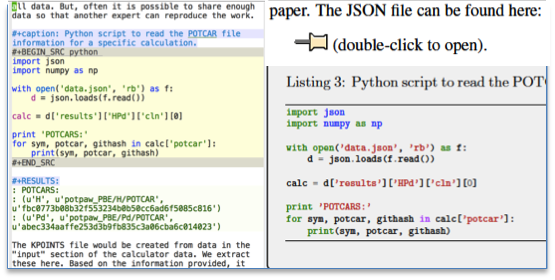
\includegraphics{TOC}
% Emacs 25.1.50.1 (Org mode 8.2.10)
\end{document}